\documentclass{beamer}



\mode<presentation> {
    \usetheme{Alife}
}

%\nonumberslides % descomentar para no numerar las diapositivas

% Comentar el campo que no desea que aparezca
\infopresentation[
    title = {(Title of the Presentation)},
    shorttitle = {(Short title of the Presentation)},
    subtitle = {(Subtitle of the Presentation)},
    author = {Author: (Name)},
    emailauthor = {(prefix)@unal.edu.co},          
    advisor = {Advisor: Jonatan Gómez Perdomo, Ph.D.},
    emailadvisor = {jgomezpe@unal.edu.co},
    coadvisor = {Coadvisor: Rodrigo De Castro Korgi, Ph.D.},
    emailcoadvisor = {rdecastrok@unal.edu.co },
    shortauthor = {(Name) \& J. Gómez},
    program = {(Doctorate/Master) in Computer Engineering},
    group = {Research Group on Artificial Life -- Grupo de 
            investigación en vida artificial -- (Alife)},
    department = {Computer and System Department},
    school = {Engineering School},
    institute = {Universidad Nacional de Colombia},
    shortinstitute = {UN},
    date  = {(1st Semester 2017)},
    logogroup = {images/logoALIFEcolor.pdf},
    logoinst = {images/Escudo_unal_2016.png},
    subject = {presentation ALIFE Group}
]

\AtBeginSection
{%
\begin{frame}<beamer>{Outline}%esquema
\tableofcontents[currentsection]%,currentsubsection
\end{frame}
}

%\AtBeginSubsection
%{%
%\begin{frame}<beamer>
%\frametitle{Contents} \tableofcontents[currentsection,currentsubsection]
%\end{frame}
%}

%\beamerdefaultoverlayspecification{<+->}

\theoremstyle{definition}
    %\newtheorem{definition}{Definition}
    \newtheorem{definitionc}{Definition (continuation)}
    %\newtheorem{definitions}{Definitions}
    \newtheorem{specification}{Specification}
    %\newtheorem{example}{Example}
    \newtheorem{examplec}{Example (continuation)}
    %\newtheorem{examples}{Examples}
\theoremstyle{theorem}
    \newtheorem{proposition}{Proposition}
    %\newtheorem{theorem}{Theorem}
    \newtheorem{theoremc}{Theorem (continuation)}
    \newtheorem{thesis}{Thesis}
    %\newtheorem{lemma}{Lemma}
    %\newtheorem{corollary}{Corollary}
    %\newtheorem*{proof}{Proof}
    \newtheorem*{proofc}{Proof (continuation)}
\theoremstyle{remark}
    \newtheorem*{remark}{Remark}
    %\newtheorem*{note}{Note}
    \newtheorem*{notes}{Notes}

\begin{document}
\renewcommand{\tablename}{Table}
\renewcommand{\figurename}{\scriptsize Figure}


\begin{frame}[plain,noframenumbering]
    \titlepage
\end{frame}

% -------------------------- Chapter 3 - Slide 4 -------------------------- % 

\begin{frame}{Agente de resolución de problemas}
    Forma restringida de un agente general:
    
    \begin{theorem}[Pseudocódigo]
        
        \begin{listing}
            {\scriptsize 
                \textcolor{darkblue}{función} \textcolor{darkred}{AGENTE-SOLUCIONADOR-DE-PROBLEMAS-SIMPLE}(\textcolor{darkgreen}{percepción}) 
                \textcolor{darkblue}{retorna} una acción
                \\* \quad\quad
                \textcolor{darkblue}{estático}: 
                \textcolor{darkgreen}{sec}, una secuencia de acciones, inicialmente vacía
                \\* \quad\quad\quad\quad\quad\quad
                \textcolor{darkgreen}{estado}, una descripción del estado actual del ambiente
                \\* \quad\quad\quad\quad\quad\quad
                \textcolor{darkgreen}{objetivo}, un objetivo, inicialmente nulo
                problema, una formulación de un problema
                \\* \quad\quad
                \textcolor{darkgreen}{estado}$\ \leftarrow $ {ACTUALIZAR-ESTADO}(
                \textcolor{darkgreen}{estado}, 
                \textcolor{darkgreen}{percepción})
                \\*\quad\quad
                \textcolor{darkblue}{si} 
                \textcolor{darkgreen}{sec} está vacío 
                \textcolor{darkblue}{entonces} 
                \\*\quad\quad\quad\quad
                \textcolor{darkgreen}{objetivo}$\ \leftarrow $ Formular-Estado(
                \textcolor{darkgreen}{estado}, 
                \textcolor{darkgreen}{percepción})
                \\*\quad\quad\quad\quad
                \textcolor{darkgreen}{problema} $\ \leftarrow $ Formular-Problema(
                \textcolor{darkgreen}{estado}, 
                \textcolor{darkgreen}{objetivo})\\*
                \quad\quad\quad\quad
                \textcolor{darkgreen}{sec} $\ \leftarrow $ Buscar(
                \textcolor{darkgreen}{problema})\\*
                \quad\quad
                \textcolor{darkgreen}{acción} $\ \leftarrow $ Recomendación(
                \textcolor{darkgreen}{sec}, 
                \textcolor{darkgreen}{estado})\\*
                \quad\quad
                \textcolor{darkgreen}{sec} $\ \leftarrow $Recordatorio(
                \textcolor{darkgreen}{sec}, 
                \textcolor{darkgreen}{estado})\\*
                \quad\quad
                \textcolor{darkblue}{retorna} acción
            }
        \end{listing}
        
    \end{theorem}
    
    {\tiny 
        \quad\quad\quad Nota: Esto es resolución de problemas de manera "\textcolor{darkgreen}{offline}"; solución ejecutada con "ojos cerrados".
        \\*\quad\quad\quad
        La solución de problemas 
        "\textcolor{darkgreen}{online}" requiere actuar con conocimiento incompleto.}
    
\end{frame}

%Slide 3

\begin{frame}{Esquema}
    \tableofcontents%[pausesections]
    %La tabla de contenidos se agrega automaticamente
    %De todos modos los títulos deben ser:
    % 1) Agentes resolventes-problemas
    % 2) Tipos de problemas
    % 3) Formulación de problemas
    % 4) Ejemplos de problemas
    % 5) Algoritmos de busqueda básica
     
\end{frame}

%slide 2

\definecolor{Green}{RGB}{0,100,0}
\begin{frame}{Recordatorios}
    \textcolor{red}{Tarea 0 hasta las 5 pm de hoy} \newline
    \textcolor{red}{Tarea 1 publicada,} 2/9 \newline
    \textcolor{Green}{sección 105 se moverá a las 9-10 am} comenzando la próxima semana
\end{frame}

\section{Agentes resolventes-problemas}%subtema

%Slide 5

\definecolor{Green}{RGB}{0,100,0}
\begin{frame}{Ejemplo: Rumania}
    Vacaciones en Rumania; actualmente en Arad.\\
    El vuelo sale mañana de Bucarest\\
    \textcolor{Green}{Formular objetivo:}\\
    \hspace{0.8cm}estar en Bucarest\\
    \textcolor{Green}{Formular problema:}\\
    \hspace{0.8cm}\textcolor{Green}{estados:} varias ciudades\\
    \hspace{0.8cm}\textcolor{Green}{acciones:} conducir entre ciudades\\
    \textcolor{Green}{Encontrar solución:}\\
    \hspace{0.8cm}secuencia de ciudades, por ejemplo, Arad, Sibiu, Fagaras, Bucarest.
\end{frame}

%Slide 6

\begin{frame}{Ejemplo: Rumanía}
    \begin{figure}
        \includegraphics[width=10cm]{6_roads_rumania.png}
    \end{figure}
\end{frame}

%Slide 7

\section{Tipos de problemas}%subtema

\begin{frame}{Tipos de problemas.}
    \textcolor{green}{Determinístico, completamente observable} $\Rightarrow$ \textcolor{blue}{problema de único estado} \newline
    \blank{1cm}El agente sabe exactamente en qué estado estará; la solución es una secuencia.
    \newline
    \textcolor{green}{No observable} $\Rightarrow$ \textcolor{blue}{estado conforme} \newline
    \blank{1cm}El agente puede no tener idea de dónde esta; la solucion (si existe) es una secuencia.
    \newline
    \textcolor{green}{No determinístico y/o parcialmente observable} $\Rightarrow$ \textcolor{blue}{problema continuos} \newline
    \blank{1cm}las percepciones proveen información \textcolor{red}{nueva} sobre el estado actual\newline
    \blank{1cm}la solución es un \textcolor{blue}{plan de contingencia} o \textcolor{blue}{una póliza}\newline
    \blank{1cm}con frecuencia una búsqueda \textcolor{red}{intercalada}, ejecución.\newlin
    \newline
    \textcolor{green}{Estado espacial desconocido} $\Rightarrow$ \textcolor{blue}{problema de exploración} (“en línea”)
\end{frame}


%slide 8

\begin{frame}{Ejemplo: mundo de una aspiradora}
    \begin{wrapfigure}{r}{0.38\textwidth} %this figure will be at the right
        \centering
        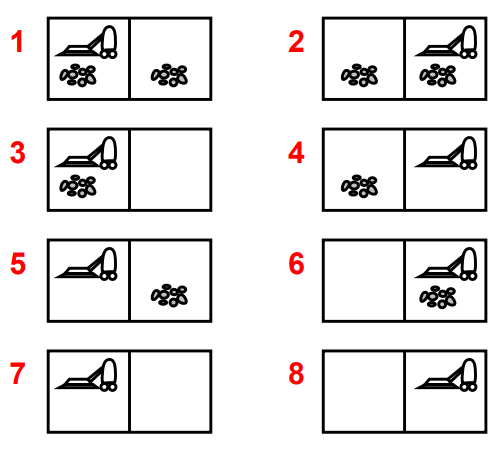
\includegraphics[width=0.35\textwidth]{8_image_example1.PNG}
    \end{wrapfigure}
    
    Estado-único, comienza en \#5. \textcolor{red}{Solución ??}
\end{frame}

% Slide 10

\begin{frame}{Ejemplo: Mundo de una aspiradora}
    \begin{columns}
        \begin{column}{0.6\textwidth}
            \emphblue{Estado-\'Unico}, comienza en \#5.
            \textcolor{red}{Solución ??}\\
            \textcolor{Pink}{$[Derecha, Aspirar]$}\\~\\
                   
            \emphblue{Conformado}, comienza en
            \textcolor{Pink}{$\{1,2,3,4,5,6,7,8\}$} e.g., \textcolor{Pink}{Derecha} va a \textcolor{Pink}{$\{2,4,6,8\}$}
            \textcolor{red}{Solución ??}\\
            \textcolor{Pink}{$[Derecha, Aspirar, Izquierda, Aspirar]$}\\~\\
                    
            \emphblue{Contingencia}, comienza en \#5.\\
            Ley de Murphy: \textcolor{Pink}{Aspirar} puede ensuciar una alfombra l\'impia.\\
            Detecci\'on local: suciedad, s\'olo por locaci\'on.
            \textcolor{red}{Soluci\'on ??}\\
                    
        \end{column}
        \begin{column}{0.4\textwidth}
            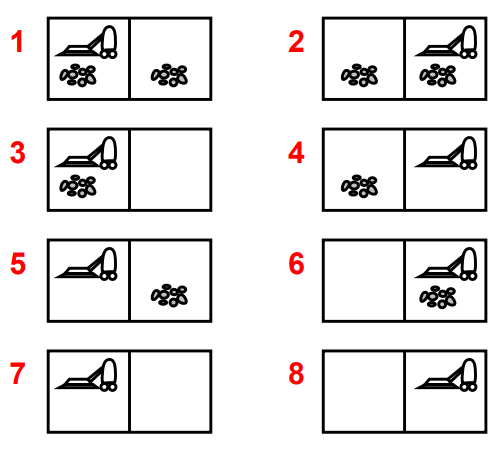
\includegraphics[width=0.8\textwidth]{9_image_example1.PNG}
        \end{column}
    \end{columns}
    
        
\end{frame}

\begin{frame}{Ejemplo: Mundo de una aspiradora}
    \begin{columns}
        \begin{column}{0.6\textwidth}
            \emphblue{Estado-\'Unico}, comienza en \#5.
            \textcolor{red}{Solución ??}\\
            \textcolor{Pink}{$[Derecha, Aspirar]$}\\~\\
                   
            \emphblue{Conformado}, comienza en
            \textcolor{Pink}{$\{1,2,3,4,5,6,7,8\}$} e.g., \textcolor{Pink}{Derecha} va a \textcolor{Pink}{$\{2,4,6,8\}$}
            \textcolor{red}{Solución ??}\\
            \textcolor{Pink}{$[Derecha, Aspirar, Izquierda, Aspirar]$}\\
                    
            \emphblue{Contingencia}, comienza en \#5.\\
            Ley de Murphy: \textcolor{Pink}{Aspirar} puede ensuciar una alfombra l\'impia.\\
            Detecci\'on local: suciedad, s\'olo por locaci\'on.
            \textcolor{red}{Soluci\'on ??}\\
            {[Derecha, \emphblue{si} suciedad \emphblue{entonces} aspirar]}
        \end{column}
        \begin{column}{0.4\textwidth}
            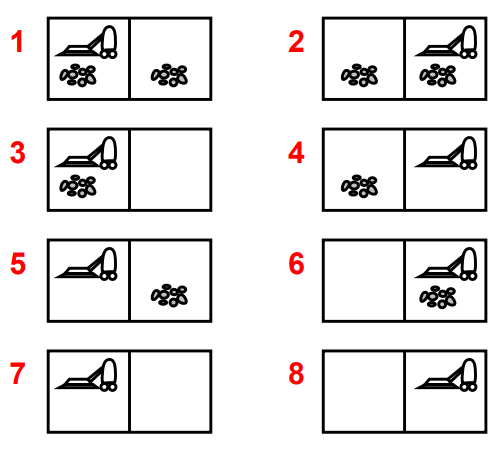
\includegraphics[width=0.8\textwidth]{9_image_example1.PNG}
        \end{column}
    \end{columns}
\end{frame}

\section{Formulación de problemas}%subtema

%Slide 12 

\begin{frame}{Formulación de problema de un Solo Estado}{Cap 3 p 12}
    \begin{right}
        
        Un problema es definido por cuatro items:
        
        - Estado inicial e.g., "at Arad"
        
        - Función Sucesora $S(x)$ = conjunto de pares de action-estado.
        
        e.g., $S(Arad)=$ \{  \left\langle Arad  \longrightarrow Zerind, Zerind \right\rangle,...\}
            
        - Prueba del objetivo, puede ser
        
        explicito, e.g., $x$ = "at Bucharest"
        
        implicito, e.g., $NoDirt(x)$
        
        - Camino de costo(aditivo)
        
        e.g., suma de distancias, numbero de acciones ejecutadas $c(x,a,y)$ es el costo del paso, asumido para ser $ \geq 0$
        
        Una solucion es una secuencia de acciones lideradas desde el estado final al estado objetivo.
        
    \end{right}
\end{frame}

%Capitulo 3 Pagina 13
\begin{frame}{Seleccionando un Espacio de estados}{Cap 3 p 13}
        
    El mundo real es absurdamente complejo \newline
    \hspace*{1em} $\Rightarrow$ El espacio de estados debe \textcolor{red}{abstraerse} para resolver el problema \newline
    (Abstracción) estado = conjunto de estados reales\newline
    (Abstracción) acción = combinacion compleja de acciones reales\newline
       
    \hspace*{1em} e.g., “Arad $\rightarrow$ Zerind” representa un conjunto complejo de posibles rutas, desvíos, parades de descanso, etc. \newline
    Para garantizar la realización, \textcolor{red}{cualquier} estado real "en Arad" debe llegar a un estado real "en Zerind"\newline
        
    (Abstracción) solución = \newline
    \hspace*{1em} conjunto de caminos reales que son soluciones en el mundo real
        
    ¡Cada acción abstracta debería ser "más fácil" que el problema original!    
        
\end{frame}

%Slide 14 
\definecolor{Pink}{RGB}{255,0,131}
\definecolor{Purple}{RGB}{166,115,255}
\definecolor{Yellow}{RGB}{224,237,0}
\definecolor{Green}{RGB}{0,100,0}

\begin{frame}{Tipos de ambiente}
    \begin{figure}\includegraphics[ width=85mm ]{16_exampleVacuum.png}\end{figure}
    \small{
        \textcolor{Pink}{\underline{¿Estados?}}:\\
        \textcolor{Pink}{\underline{¿Acciones?}}:\\
        \textcolor{Pink}{\underline{¿Estado objetivo?}}:\\
        \textcolor{Pink}{\underline{¿Costo de ruta?}}: 
    }
    \break\break\break\break\break
\end{frame}

\definecolor{Pink}{RGB}{255,0,131}
\definecolor{Purple}{RGB}{166,115,255}
\definecolor{Yellow}{RGB}{224,237,0}
\definecolor{Green}{RGB}{0,100,0}

% Pagina 16%
\begin{frame}{Tipos de ambiente}
    \begin{figure}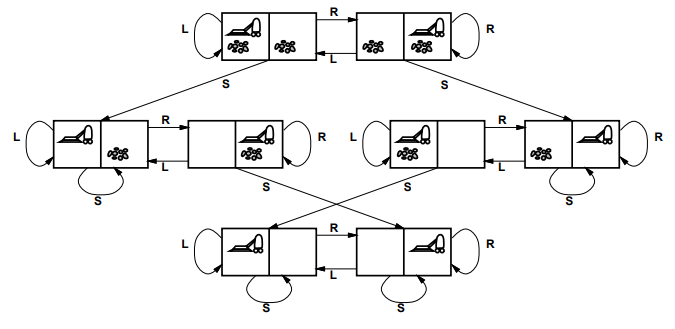
\includegraphics[ width=85mm ]{15_exampleVacuum.png}\end{figure}
    \small{
        \textcolor{Pink}{\underline{¿Estados?}}: Suciedad como entero y ubicacion del robot \\          \hspace{1.8cm} (ignore las \textcolor{Green}{cantidades} de suciedad, etc.) \\
        \textcolor{Pink}{\underline{¿Acciones?}}: \\
        \textcolor{Pink}{\underline{¿Estado objetivo?}}: \\
        \textcolor{Pink}{\underline{¿Costo de ruta?}}: 
    }
    \break\break\break\break\break
\end{frame}


%Slide 16

\definecolor{Pink}{RGB}{255,0,131}
\definecolor{Purple}{RGB}{166,115,255}
\definecolor{Yellow}{RGB}{224,237,0}
\definecolor{Green}{RGB}{0,100,0}

% Pagina 16%
\begin{frame}{Tipos de ambiente}
    \begin{figure}\includegraphics[ width=85mm ]{16_exampleVacuum.png}\end{figure}
    \small{
        \textcolor{Pink}{\underline{¿Estados?}}: Suciedad como entero y ubicacion del robot \\          \hspace{1.8cm} (ignore las \textcolor{Green}{cantidades} de suciedad, etc.) \\
        \textcolor{Pink}{\underline{¿Acciones?}}: \textcolor{Purple}{$Izquierda, Derecha, Aspirar, %
            Sin \hspace{0.1cm}acciones$} \\
        \textcolor{Pink}{\underline{¿Estado objetivo?}}: \\
        \textcolor{Pink}{\underline{¿Costo de ruta?}}: 
    }
    \break\break\break\break\break
\end{frame}

\definecolor{Pink}{RGB}{255,0,131}
\definecolor{Purple}{RGB}{166,115,255}
\definecolor{Yellow}{RGB}{224,237,0}
\definecolor{Green}{RGB}{0,100,0}

% Pagina 16%
\begin{frame}{Tipos de ambiente}
    \begin{figure}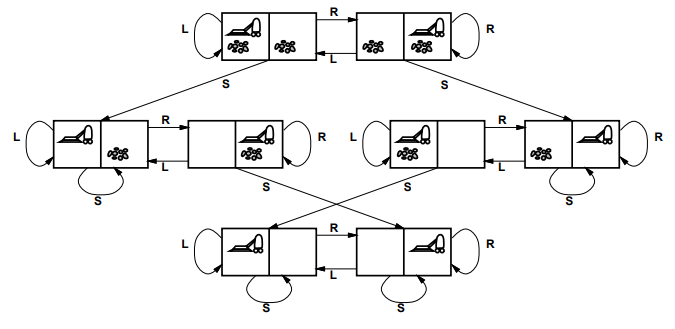
\includegraphics[ width=85mm ]{17_exampleVacuum.png}\end{figure}
    \small{
        \textcolor{Pink}{\underline{¿Estados?}}: Suciedad como entero y ubicacion del robot \\          \hspace{1.8cm} (ignore las \textcolor{Green}{cantidades} de suciedad, etc.) \\
        \textcolor{Pink}{\underline{¿Acciones?}}: \textcolor{Purple}{$Izquierda, Derecha, Aspirar, %
            Sin \hspace{0.1cm}acciones$} \\
        \textcolor{Pink}{\underline{¿Estado objetivo?}}: Sin suciedad \\
        \textcolor{Pink}{\underline{¿Costo de ruta?}}: 
    }
    \break\break\break\break\break
\end{frame}

%pagina 20 
\begin{frame}{Ejemplo: El "8-Puzzle"}
    \begin{figure}
        \centering
        \includegraphics[scale=0.7]{20_image_cap3pag20.PNG}
        \begin{flushleft}
            \\ \textcolor{purple}{Estados??} ubicaciones enteras de casillas (ignorar posiciones intermedias)
            \\\textcolor{purple}{Acciones??}
            \\\textcolor{purple}{Prueba de Objetivo??}
            \\\textcolor{purple}{Costo del Camino??}
        \end{flushleft}
    \end{figure}{}
        
\end{frame}

%Capitulo 3, presentación 21
\definecolor{Pink}{RGB}{255,0,131}
\begin{frame}{Ejemplo: Juego del 8}
    \begin{columns}
        \begin{column}{0.5\textwidth}       
            \begin{figure}[h!]
                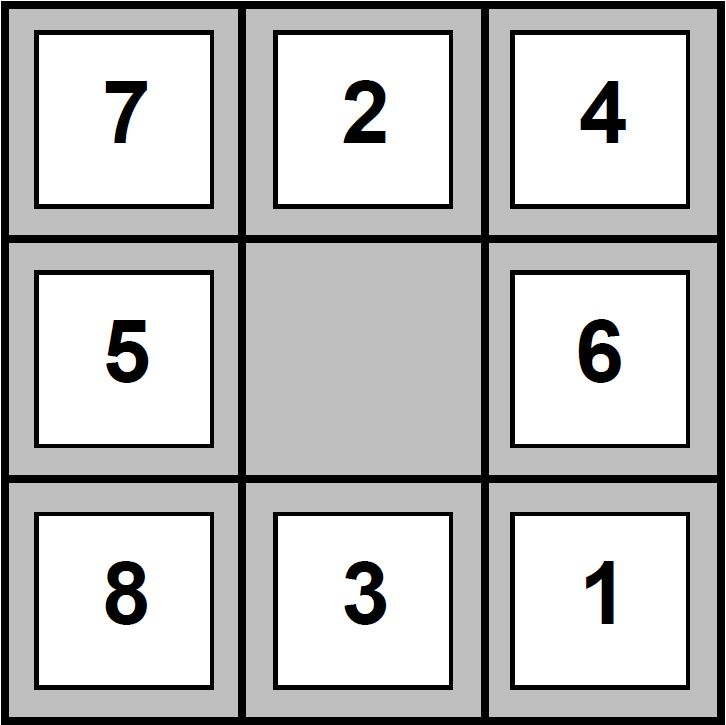
\includegraphics[scale=.15]{21_grid1.JPG}
                \\
                \vspace{0pt}
                {\tiny Estado Inicial}
            \end{figure}
        \end{column}
                
        \begin{column}{0.5\textwidth}  %%<--- here
            \begin{figure}
                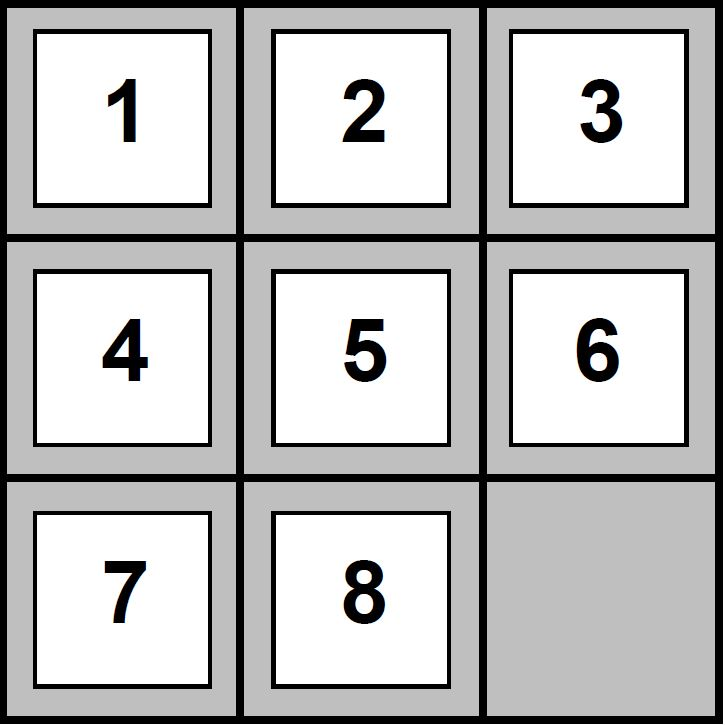
\includegraphics[scale=.15]{21_grid2.JPG}
                \\
                \vspace{0pt}
                {\tiny Estado Objetivo}
            \end{figure}
        \end{column}
    \end{columns}
    \vfill
    \small{ 
        \textcolor{Pink}{\underline{¿Estados?}}: ubicaciones enteras de las casillas (ignorar posiciones intermedias)\\
        \textcolor{Pink}{\underline{¿Acciones?}}: mover a una casilla vacia a la izquierda, derecha, arriba, abajo (ignorar desajustes etc.)\\
        \textcolor{Pink}{\underline{¿Estado objetivo?}}\\
        \textcolor{Pink}{\underline{¿Costo de ruta?}}\\
    }
\end{frame}

%CAPITULO 3
%pagina 23 
\begin{frame}{Ejemplo: El "8-Puzzle"}
    \begin{figure}
        \centering
        \includegraphics[scale=0.7]{20_image_cap3pag20.PNG}
        \begin{flushleft}
            \\ \textcolor{purple}{Estados??} ubicaciones enteras de casillas (ignorar posiciones intermedias)
            \\\textcolor{purple}{Acciones??}
            \\\textcolor{purple}{Prueba de Objetivo??}
            \\\textcolor{purple}{Costo del Camino??} 1 Por Movimiento
                    
            [Note: optimal solution of n-Puzzle family is NP-hard]
        \end{flushleft}
    \end{figure}{}
        
\end{frame}

%Chap 3 pag 24
\definecolor{Pink}{RGB}{255,0,131}
\definecolor{DarkRed}{RGB}{128,0,0}

\begin{frame}{Ejemplo: Ensamblaje robótico}
    \begin{figure}
        \centering
        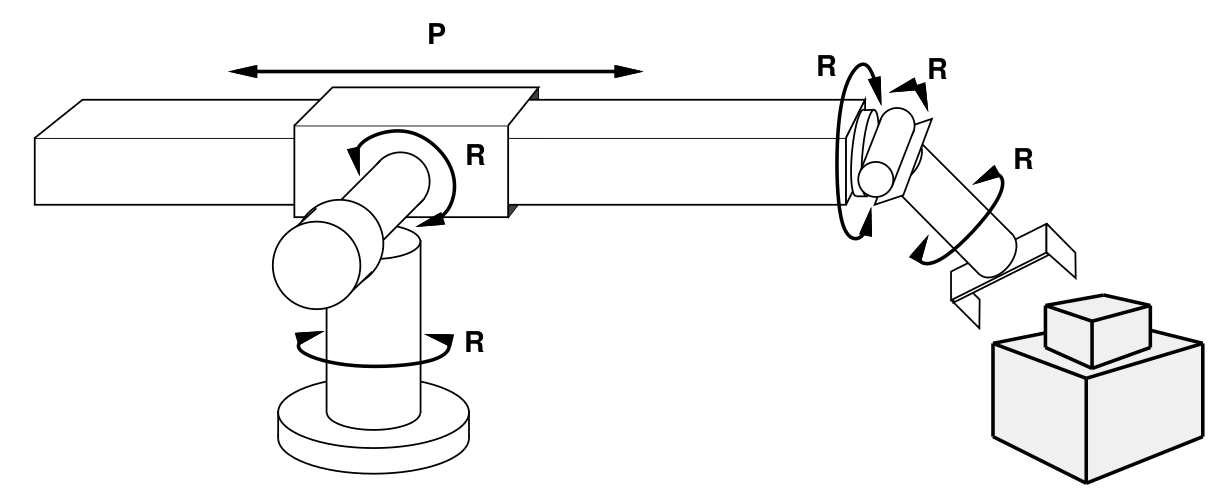
\includegraphics[scale=0.23]{24_chap3_pag24.png}
    \end{figure}
    \begin{flushleft}
        \textcolor{Pink}{¿Estados?}: Coordenadas, en valores reales, de los ángulos de unión de las partes del objeto a ensamblar.\\
        \textcolor{Pink}{¿Acciones?}: Movimientos continuos de las articulaciones del
        robot.\\
        \textcolor{Pink}{¿Estado de Objetivo?}: Montaje completo,
        \textcolor{DarkRed}{¡sin robot incluido!}\\
        \textcolor{Pink}{¿Costo de ruta?}: Tiempo de ejecución.
    \end{flushleft}
\end{frame}

%slide 26
\begin{frame}{Ejemplo árbol de búsqueda}{}
    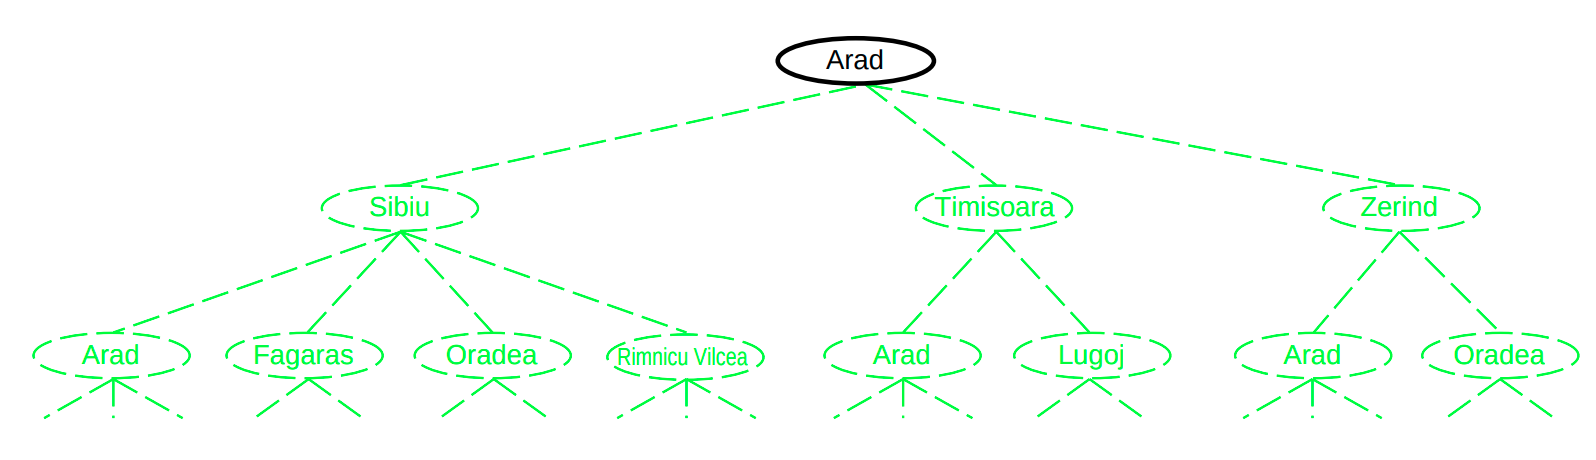
\includegraphics[scale=0.2]{26_chap3_pag26.png}
\end{frame}

%Chap 3 pag 27
\begin{frame}{Ejemplo árbol de búsqueda}{}
    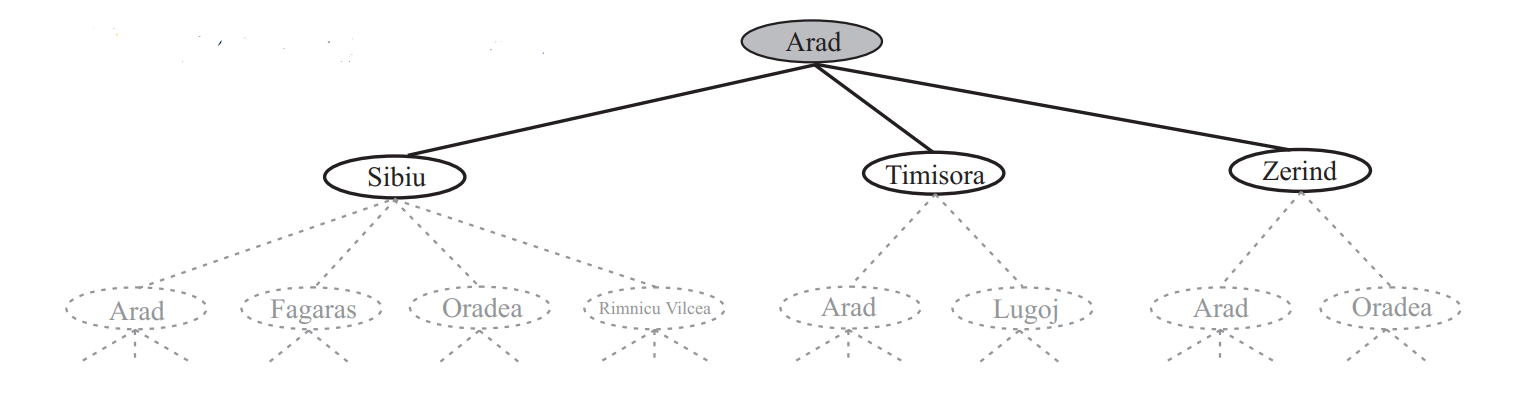
\includegraphics[scale =0.3]{chap3-pag27.PNG}
    
\end{frame}

%slide 28
\begin{frame}{Ejemplo árbol de búsqueda}
    \begin{figure}
        \centering
        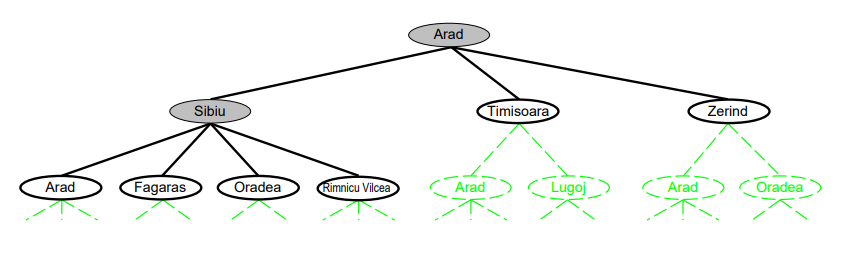
\includegraphics[width = 112mm, scale = 1]{Chapter3Slide28.png}
    \end{figure}
    
\end{frame}


%Chap 3 pag 29
\definecolor{DarkRed}{RGB}{128,0,0}
\definecolor{Green}{RGB}{0,100,0}
\begin{frame}{Implementación: estados vs. nodos}
    Un \textcolor{blue}{estado} es una (representación de) una configuración física\\
    Un \textcolor{blue}{nodo} es una estructura de datos que constituye parte de un árbol de búsqueda que incluye \textcolor{Green}{padre}, \textcolor{Green}{hijos}, \textcolor{Green}{profundidad}, \textcolor{Green}{costo de ruta} \textcolor{DarkRed}{g(x)}.\\
    ¡Los estados no tienen padres, hijos, profundidad o costo de ruta!
    \begin{figure}
        \centering
        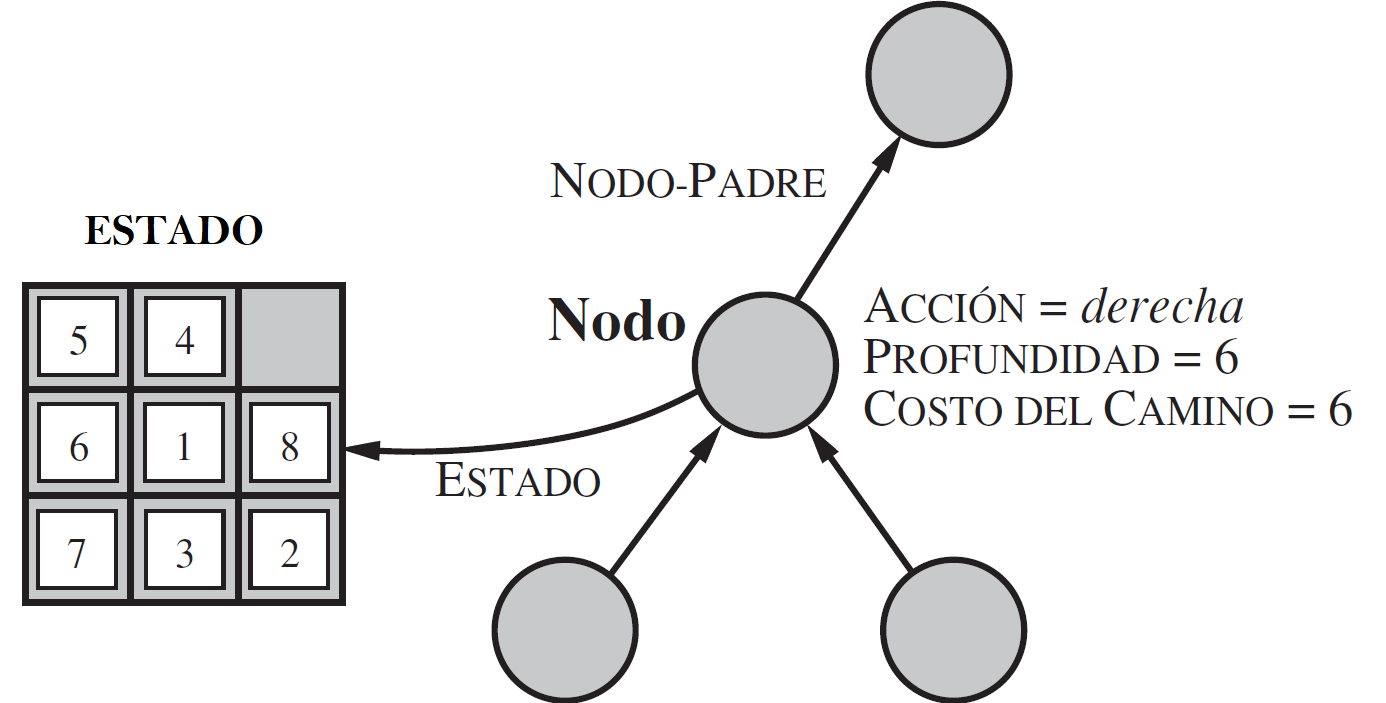
\includegraphics[width = 60mm, scale = 0.7]{29_image.PNG}
    \end{figure}
    La función \rmfamily{\textit{Expand}} crea nuevos nodos, completando los diversos campos\\
    \hspace{0.8cm}y usando el \rmfamily{\textit{SuccessorFn}} del problema para crear los\\
    \hspace{0.8cm}estados correspondientes.
\end{frame}

%% slide  30
\begin{frame}{Impementación: Árbol de búsqueda general}
    \begin{right}
        
        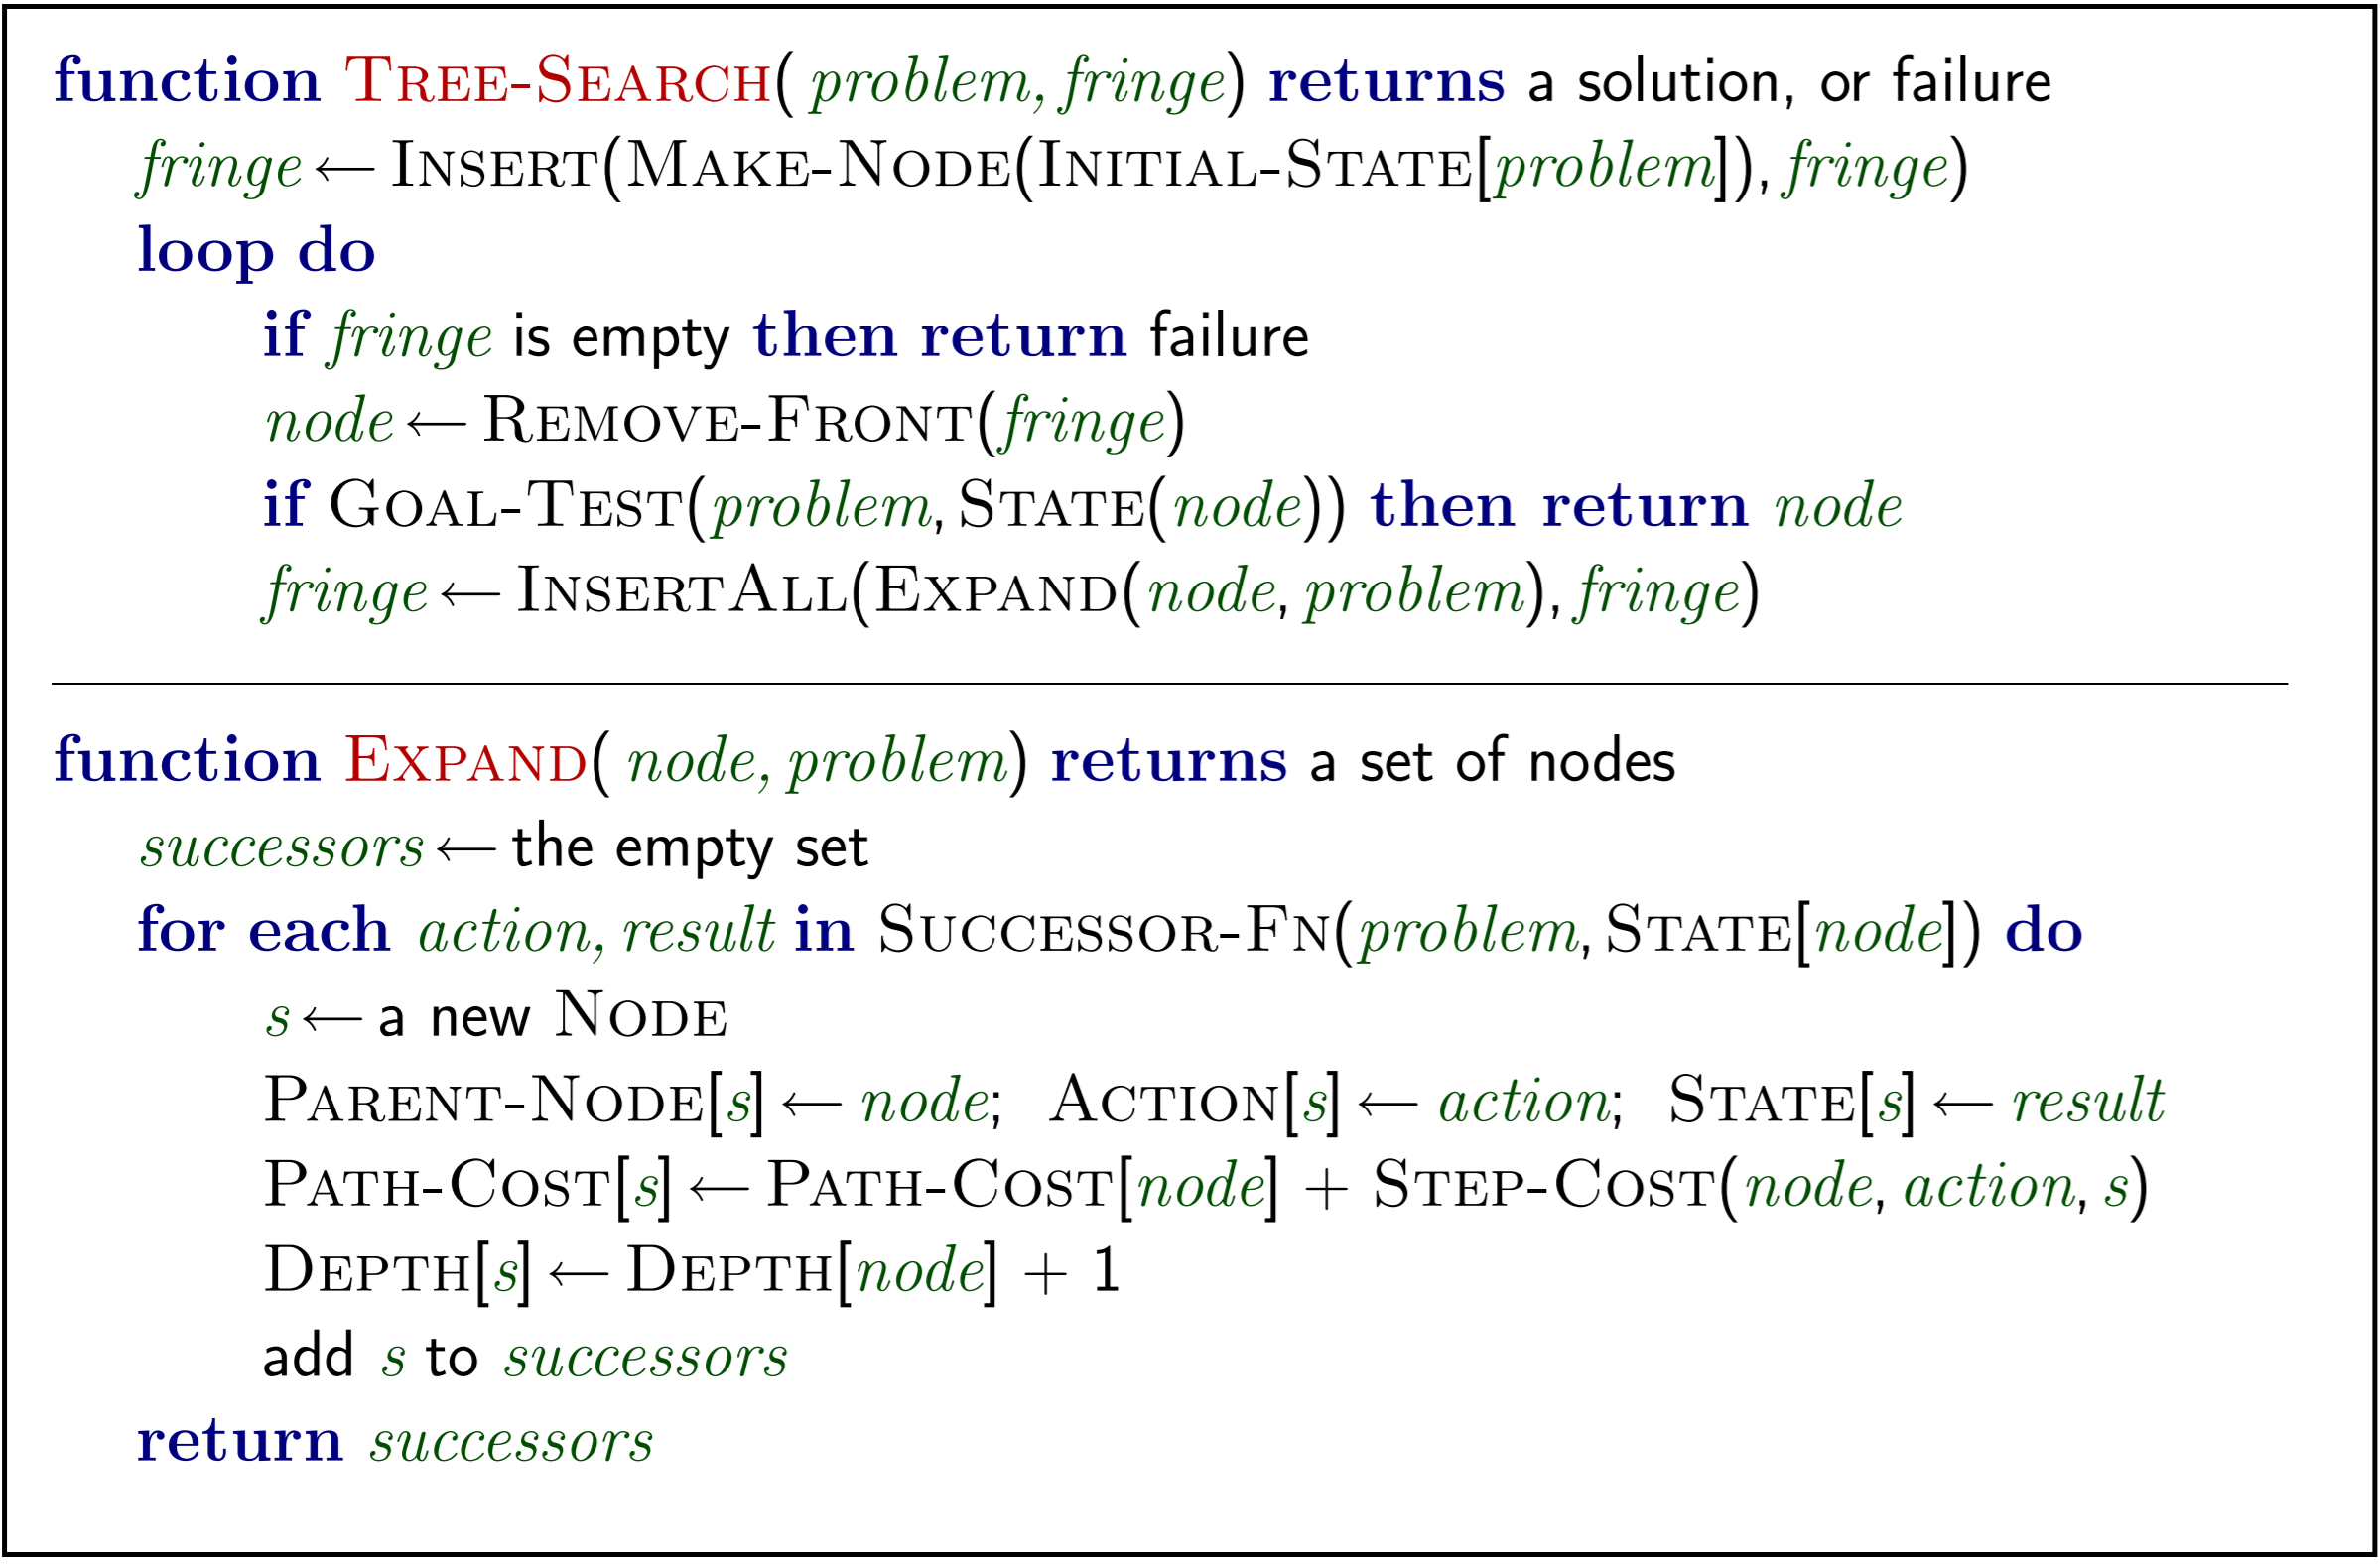
\includegraphics[scale = 0.5]{30_general_tree_search.png}
        
    \end{right}
\end{frame}

%slide 31
\begin{frame}{Estrategias de búsqueda}
    Una estrategia es definida como escoger un  \textcolor{red}{orden de los nodos de expansión.} \newline
    Las estrategias son evaluadas a partir de las siguientes parametros:\newline
    \blank{1cm}\textcolor{blue}{completitud} $-$ si existe ¿siempre encuentra la solución? \newline
    \blank{1cm}\textcolor{blue}{complejidad temporal} $-$ número de nodos generados/expandidos\newline
    \blank{1cm}\textcolor{blue}{complejidad espacial} $-$ máximo número de nodos en memoria.\newline
    \blank{1cm}\textcolor{blue}{óptimo} $-$ ¿siempre encuentra la solución menos costosa?\newline
    las complejidades temporales y espaciales se miden en términos de\newline
    \blank{1cm}\textcolor{pink}{$b$} $-$ actor máximo de ramificación en el árbol de búsqueda
    \newline
    \blank{1cm}\textcolor{pink}{$d$}$-$ máximo número de nodos en memoria.\newline
    \blank{1cm}\textcolor{pink}{$m$}$-$ profundidad máxima de los estados en el espacio (puede ser $\infty$).\newline
\end{frame}

% slide 32
\begin{frame}{Estrategias de búsqueda desinformadas}
    
      
    Las estrategias \textcolor{blue}{desinformadas} usan solo la información disponible en la definición del problema.
    \bigskip
    \bigskip
        
    Búsqueda primero en anchura.
    \bigskip
        
    Búsqueda de costo uniforme.
    \bigskip
        
    Búsqueda primero en profundidad.
    \bigskip
        
    Búsqueda de profundidad limitada.
    \bigskip
        
    Búsqueda primero en profundidad con profundidad iterativa.
    
        
\end{frame}

%Slide 34
\begin{frame}{B\'usqueda primero en anchura}
    Expandir el nodo sin expandir de menor profundidad\\~\\
    \emphblue{Implementaci\'on}:\\
    \quad\textcolor{red}{\textit{la frontera}} es una cola FIFO, i.e., los nuevos sucesores van al final
    \centering
    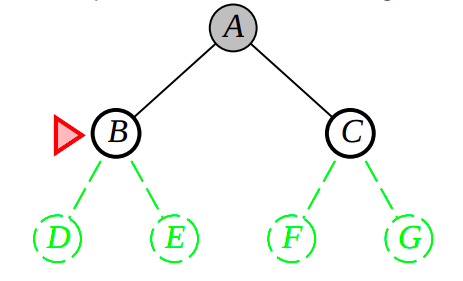
\includegraphics[width=0.5\textwidth]{34_image_bfs2.PNG}
    
\end{frame}

%sldie 35

\begin{frame}{B\'usqueda primero en anchura}
    Expandir el nodo sin expandir de menor profundidad\\~\\
    \emphblue{Implementaci\'on}:\\
    \quad\textcolor{red}{\textit{la frontera}} es una cola FIFO, i.e., los nuevos sucesores van al final
    \centering
    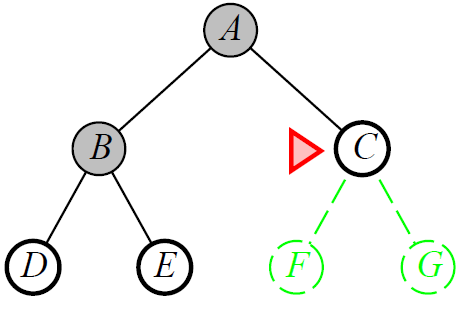
\includegraphics[width=0.5\textwidth]{35_image_bfs2.PNG}
    
\end{frame}

%% Paginas 36 Cap 3 #############################################################################################
\begin{frame}{Breadth-first search}{Cap 3 p 36}
    \begin{right}
        
        Ir al nodo no expandido mas profundo
        Implementacion:
        $fringe$ es una cola FIFO, i.e., nuevos sucesores fan al final
        
        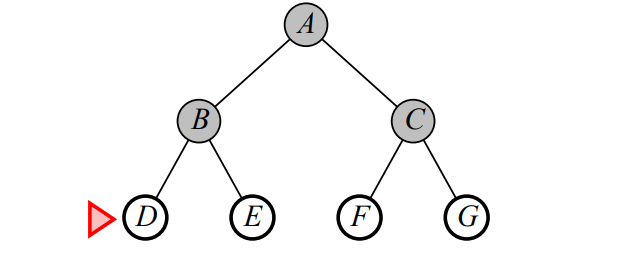
\includegraphics[scale = 0.5]{tree_bfs_p36.PNG}
        
    \end{right}
\end{frame}

%Capitulo 3 Pagina 37
\begin{frame}{Propiedades de la búsqueda de amplitud}{Cap 3 p 37}
    \textcolor{Pink}{¿Completo?}
\end{frame}

%Capitulo 3 Pagina 38%
\begin{frame}{Propiedades de la búsqueda de amplitud}
    \textcolor{Pink}{¿Completo?} Si, sí \textcolor{Purple}{$b$} es finito \\
    \textcolor{Pink}{¿Tiempo?}
\end{frame}

% Pagina 39%
\begin{frame}{Propiedades de la búsqueda de amplitud}
    \textcolor{Pink}{¿Completo?} Si, sí \textcolor{Purple}{$b$} es finito \\
    \textcolor{Pink}{¿Tiempo?} \textcolor{Purple}{$1+b^2+b^3+...+b^d+b(b^d-1)=O(b^{d+1})$} es decir,\\    \hspace{9.3cm} exponecial en \textcolor{Purple}{$d$} \\
    \textcolor{Pink}{¿Espacio?} \\
\end{frame}

%slide 40
\begin{frame}{Propiedades de la búsqueda de amplitud}
    \textcolor{Pink}{¿Completo?} Si, sí \textcolor{Purple}{$b$} es finito \\
    \textcolor{Pink}{¿Tiempo?} \textcolor{Purple}{$1+b^2+b^3+...+b^d+b(b^d-1)=O(b^{d+1})$} es decir,\\    \hspace{9.3cm} exponecial en \textcolor{Purple}{$d$} \\
    \textcolor{Pink}{¿Espacio?} \textcolor{Purple}{$O(b^{d+1})$}, mantiene todos los nodos en memoria \\
    \textcolor{Pink}{¿Óptimo?}
\end{frame}

%sldie 41
\begin{frame}{Propiedades de la búsqueda de amplitud}
    \textcolor{Pink}{¿Completo?} Si, sí \textcolor{Purple}{$b$} es finito \\
    \textcolor{Pink}{¿Tiempo?} \textcolor{Purple}{$1+b^2+b^3+...+b^d+b(b^d-1)=O(b^{d+1})$} es decir,\\    \hspace{9.3cm} exponecial en \textcolor{Purple}{$d$} \\
    \textcolor{Pink}{¿Espacio?} \textcolor{Purple}{$O(b^{d+1})$}, mantiene todos los nodos en memoria \\
    \textcolor{Pink}{¿Óptimo?} Si (Si el costo es de 1 por paso); en general no es optimo \\
    El espacio es el gran problema; puede generar nodos fácilmente a 100MB/sec\\
    entonces 24 horas = 8640 GB. \\
\end{frame}

%pagina 44
\begin{frame}{Busqueda "Deph-First"}
        
    Expandir el nodo no expandido mas profundo
    \\\textcolor{red}{\large{Implementacion:}}
    \\\qquad\qquad\textit{fringe:} Cola LIFO, es decir , poner el sucesor al frente
    \\
    \centering
    \includegraphics[scale=0.5]{44_image_cap3pag44.PNG}
        
\end{frame}

%Capitulo 3, presentación 45
\definecolor{Red}{RGB}{100,10,10}
\definecolor{DarkGreen}{RGB}{10,100,10}
\begin{frame}{Busqueda "Deph-First"}
    Expandir el nodo no expandido más profundo
    \\
    \textcolor{Red}{\large{Implementación:}}
    \\
    \qquad\qquad\textcolor{DarkGreen}{\textit{fringe}} = Cola LIFO, es decir , poner el sucesor al frente
    \\
    \centering
    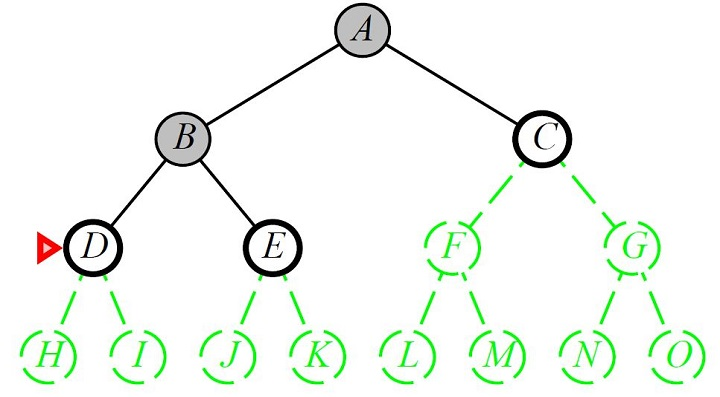
\includegraphics[scale=.5]{43_tree.JPG} 
\end{frame}

%pagina 47
\begin{frame}{Busqueda "Deph-First"}
        
    Expandir el nodo no expandido mas profundo
    \\\textcolor{red}{\large{Implementacion:}}
    \\\qquad\qquad\textit{fringe:} Cola LIFO, es decir , poner el sucesor al frente
    \\
    \centering
    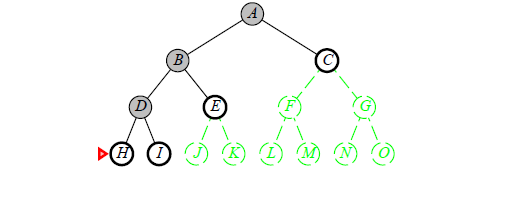
\includegraphics[scale=0.5]{47_image_cap3pag47.PNG}
        
\end{frame}

%Chap 3 pag 48
\definecolor{DarkRed}{RGB}{128,0,0}
\definecolor{Green}{RGB}{0,100,0}

\begin{frame}{Búsqueda en profundidad}
    Expandir el nodo no expandido más profundo.\\
    \begin{center}
        \textit{\textcolor{Green}{franja}} = cola LIFO, es decir, poner sucesores al
        frente.\\
    \end{center}{}
    
    \textcolor{DarkRed}{Implementación:}
    \begin{figure}
        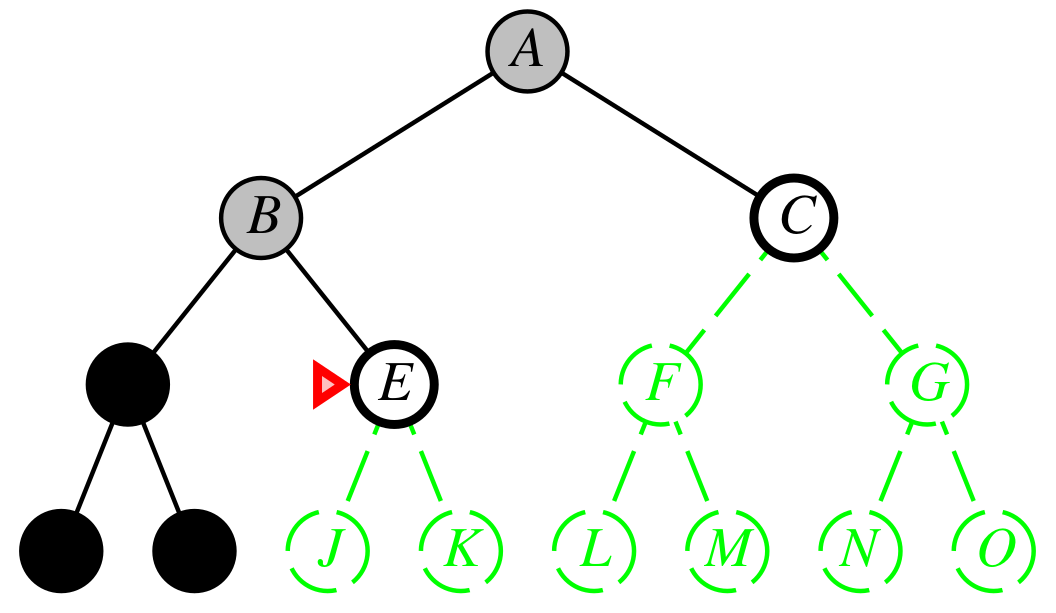
\includegraphics[scale=0.2]{48_chap3_pag48.png}
    \end{figure}
\end{frame}{}

%slide 50

\definecolor{DarkRed}{RGB}{128,0,0}
\definecolor{Green}{RGB}{0,100,0}
\begin{frame}{Búsqueda en profundidad}
    Expandir el nodo no expandido más profundo.\\
    \textcolor{DarkRed}{Implementación:}
    \begin{center}
        \textit{\textcolor{Green}{franja}} = cola LIFO, es decir, poner sucesores al
        frente.\\
    \end{center}
    \begin{figure}
        \centering
        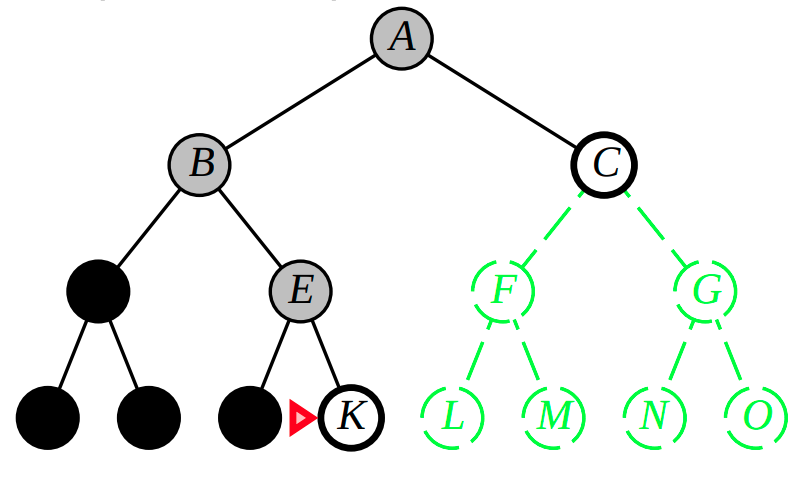
\includegraphics[width = 60mm, scale = 0.7]{50_chap3_pag50.PNG}
    \end{figure}
\end{frame}

%Chap 3 pag 51
\definecolor{DarkRed}{RGB}{128,0,0}
\definecolor{Green}{RGB}{0,100,0}

\begin{frame}{Búsqueda en profundidad}
    Expandir el nodo no expandido más profundo.\\
    \begin{center}
        \textit{\textcolor{Green}{franja}} = cola LIFO, es decir, poner sucesores al
        frente.\\
    \end{center}{}
    
    \textcolor{DarkRed}{Implementación:}
    \begin{figure}
        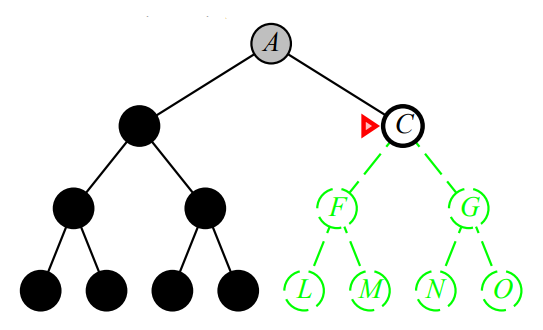
\includegraphics[scale=0.2]{51_chap3_pag51.png}
    \end{figure}
\end{frame}{}

%Chap 3 pag 53
\definecolor{DarkRed}{RGB}{128,0,0}
\definecolor{Green}{RGB}{0,100,0}
\begin{frame}{Búsqueda en profundidad}
    Expandir el nodo no expandido más profundo.\\
    \textcolor{DarkRed}{Implementación:}
    \begin{center}
        \textit{\textcolor{Green}{franja}} = cola LIFO, es decir, poner sucesores al
        frente.\\
    \end{center}
    \begin{figure}
        \centering
        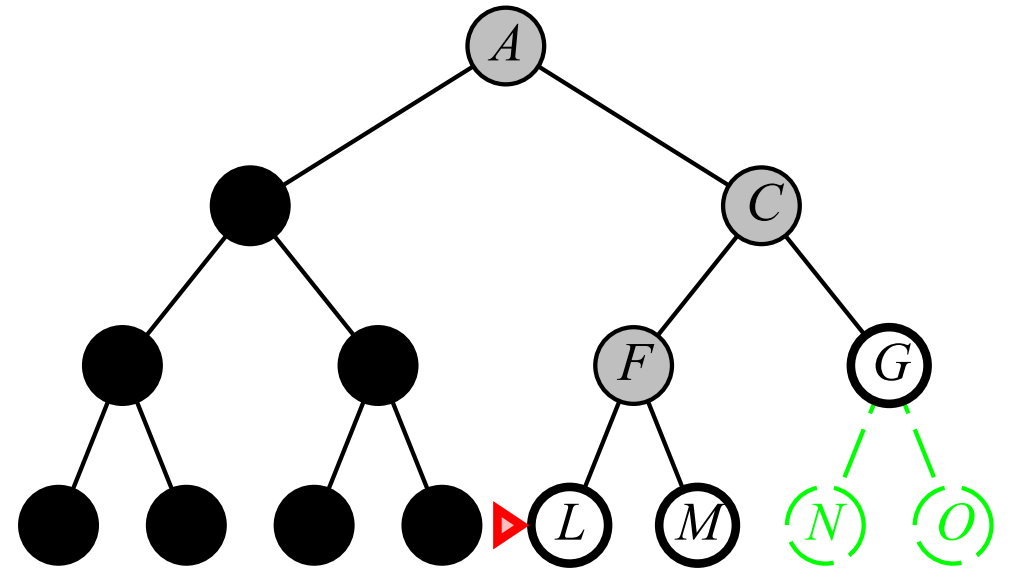
\includegraphics[width = 60mm, scale = 0.7]{53_image.PNG}
    \end{figure}
\end{frame}{}

%Chap 3 pag 54
\definecolor{DarkRed}{RGB}{128,0,0}
\definecolor{Green}{RGB}{0,100,0}
\begin{frame}{Búsqueda en profundidad}
    Expandir el nodo no expandido más profundo.\\
    \textcolor{DarkRed}{Implementación:}
    \begin{center}
        \textit{\textcolor{Green}{franja}} = cola LIFO, es decir, poner sucesores al
        frente.\\
    \end{center}
    \begin{figure}
        \centering
        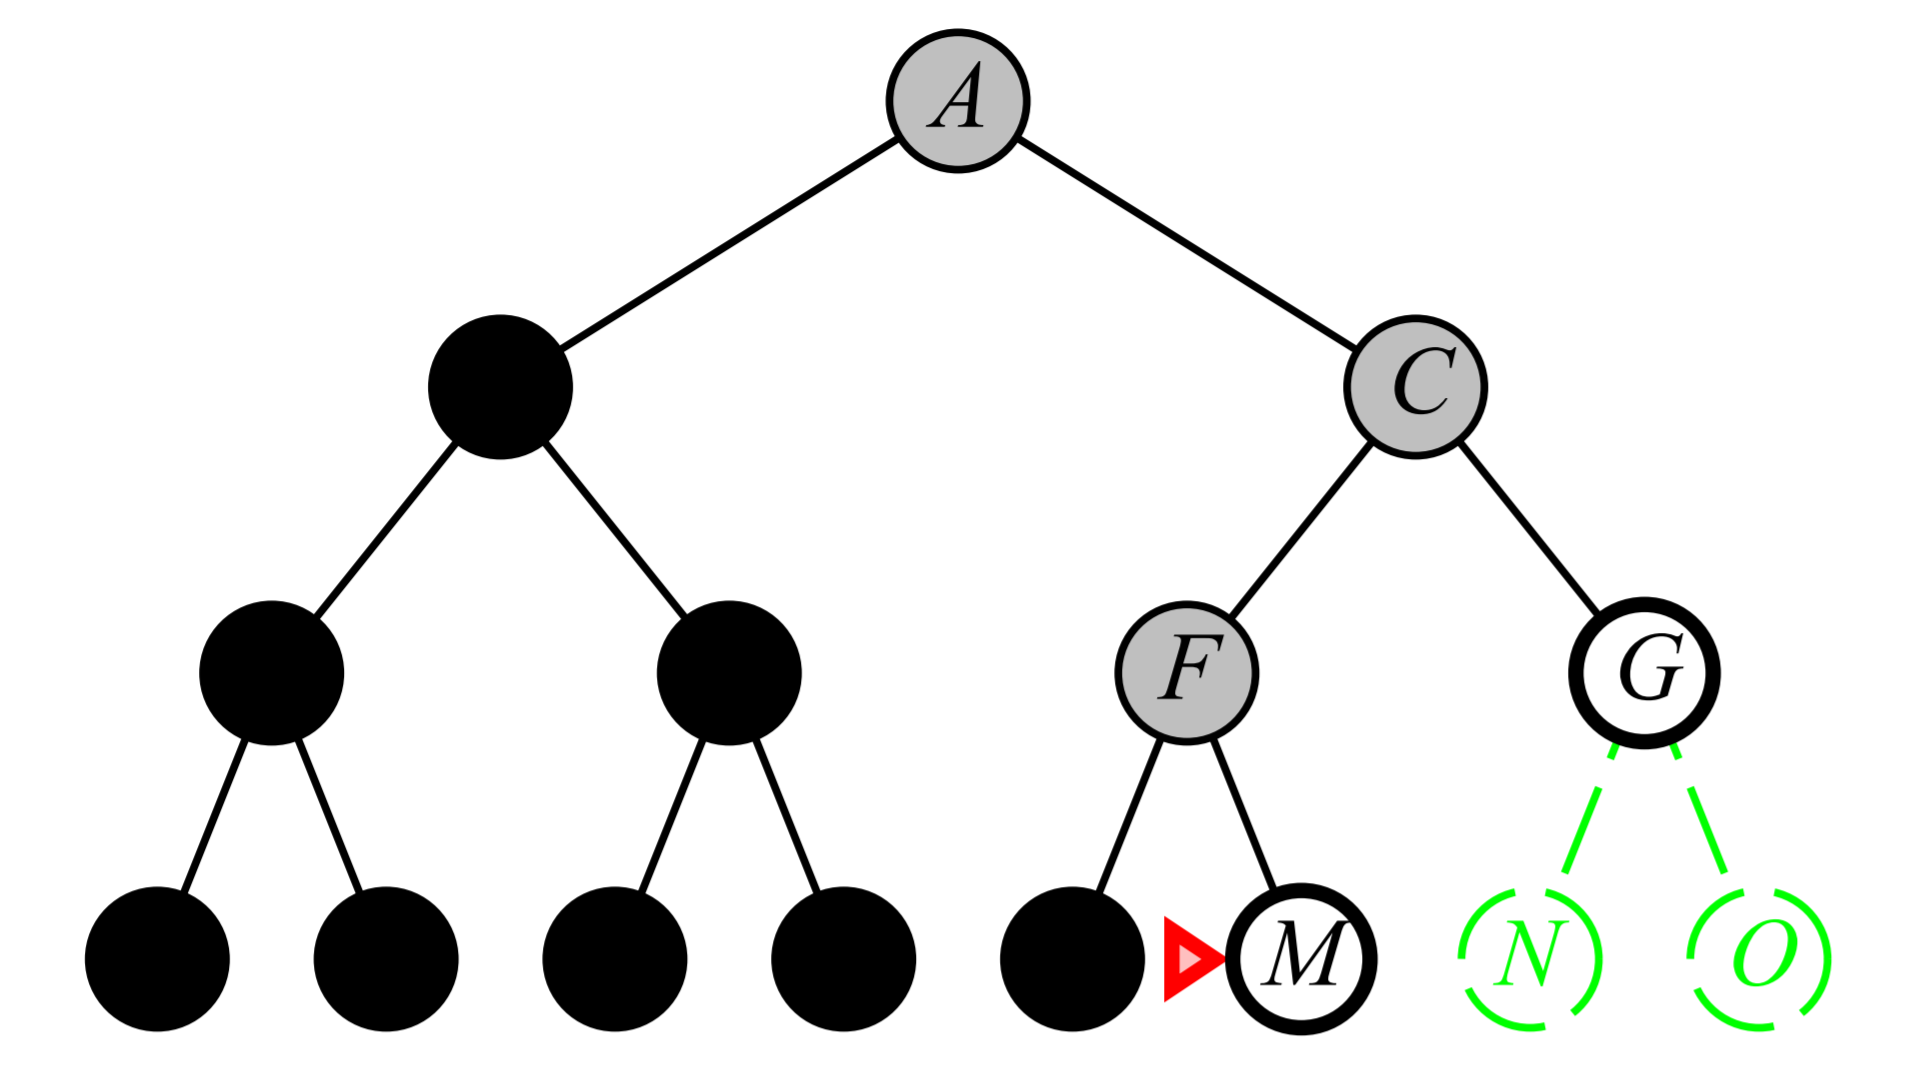
\includegraphics[width = 60mm, scale = 0.7]{54_image.PNG}
    \end{figure}
\end{frame}{}


% Slide 55
\begin{frame}{Propiedad en la búsqueda a profundidad}
    \textcolor{pink}{\underline{¿Es completa?}}
\end{frame}

%slide 56

\begin{frame}{Propiedades de búsqueda primero en profundidad}
    
      
    \textcolor{red}{Completa??} No: falla en espacios de profundidad infinita, espacios con bucles
        
    \quad \quad \quad Modificar para evitar estados repetidos a lo largo de la ruta
        
    \quad \quad \quad \quad \quad $\Rightarrow$ completa en espacios finitos
    \bigskip
        
    \textcolor{red}{Tiempo??}
        
\end{frame}

%slide 58
\begin{frame}{Propiedades de la b\'usqueda primero en profundidad}
    \emphblue{\underline{Completo}??} No: falla in espacios infinitamente profundos, espacios con ciclos.\\
    \quad Modificar para evadir estados repetidos a lo largo del camino\\
    \quad $\Rightarrow$ completo en espacios finitos\\~\\
        
    \emphblue{\underline{Tiempo}?? $O(b^m)$}: terrible si \emphblue{$m$} es mucho m\'as largo que \emphblue{$d$}\\
    \quad pero si las soluciones son densas, debe ser m\'as r\'apida que primero en anchura\\~\\
        
    \emphblue{\underline{Espacio}?? $O(bm)$}, i.e., Espacio lineal!\\
    \emphblue{\underline{\'Optimo}??}
    
\end{frame}

%slide 59

\begin{frame}{Propiedades de la b\'usqueda primero en profundidad}
    \emphblue{\underline{Completo}??} No: falla in espacios infinitamente profundos, espacios con ciclos.\\
    \quad Modificar para evadir estados repetidos a lo largo del camino\\
    \quad $\Rightarrow$ completo en espacios finitos\\~\\
        
    \emphblue{\underline{Tiempo}?? $O(b^m)$}: terrible si \emphblue{$m$} es mucho m\'as largo que \emphblue{$d$}\\
    \quad pero si las soluciones son densas, debe ser m\'as r\'apida que primero en anchura\\~\\
        
    \emphblue{\underline{Espacio}?? $O(bm)$}, i.e., Espacio lineal!\\
    \emphblue{\underline{\'Optimo}??} No
    
\end{frame}

%% Paginas 60 Cap 3 #############################################################################################
\begin{frame}{Depth-limited search}{Cap 3 p 60}
    \begin{right}
        
        = la busqueda de DFS con un limite de profundidad $l$
        
        i.e., nodo a la profundidad $l$ no tienen sucesores
        
        Implementacion recursiva:
        
        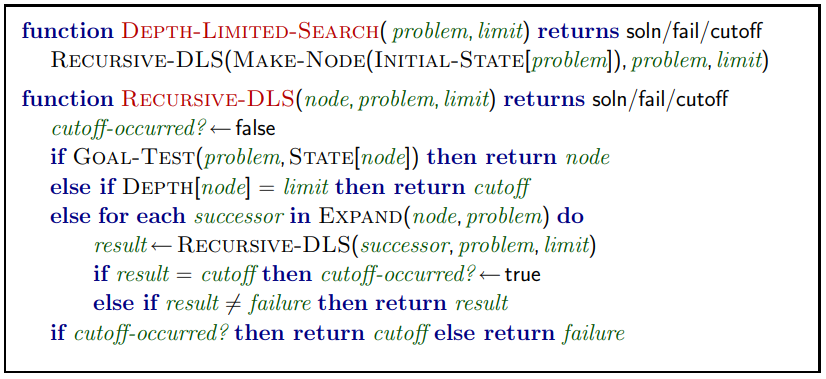
\includegraphics[scale = 0.5]{dfs_limit.PNG}
        
    \end{right}
\end{frame}

%Capitulo 3 Pagina 61
\begin{frame}{Busqueda de Profundidad Iterativa}{Cap 3 p 60}
    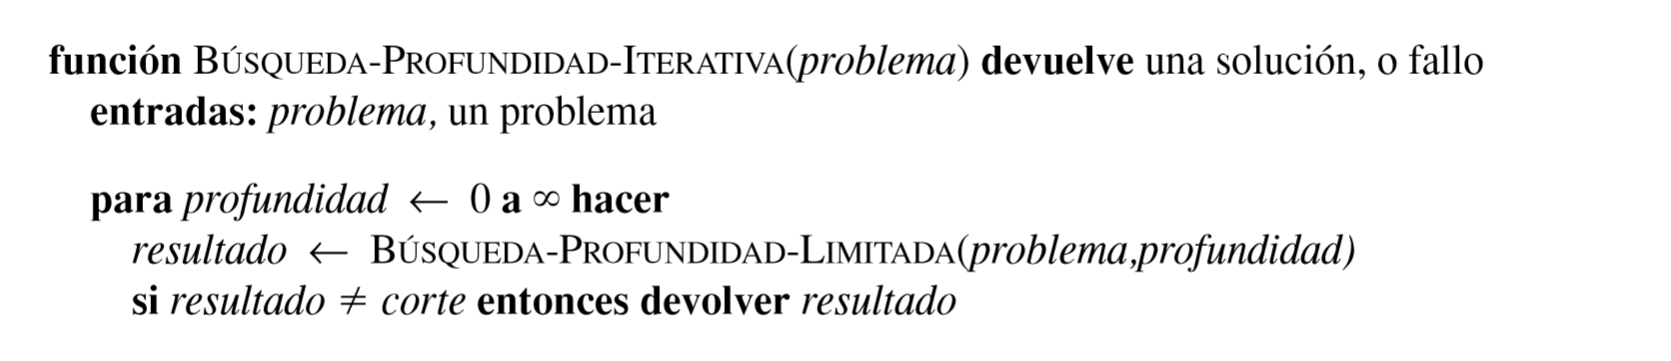
\includegraphics[scale = 0.35]{61_dfsIterativo.PNG}
\end{frame}

%Capitulo 3 Pagina 62%
\begin{frame}{Búsqueda de profundización iterativa \textcolor{Yellow}{$l=0$}}
    Limite = 0
    \begin{figure}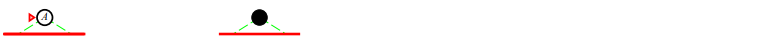
\includegraphics[width =123mm]{62_IDS_l0.PNG}\end{figure}
\end{frame}
    
% Pagina 63%
\begin{frame}{Búsqueda de profundización iterativa \textcolor{Yellow}{$l=1$}}
    Limite = 1
    \begin{figure}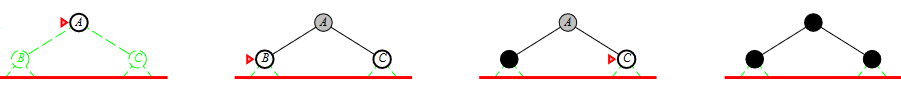
\includegraphics[width =123mm]{63_IDS_l1.png}\end{figure}
\end{frame}

% Pagina 64%
\begin{frame}{Búsqueda de profundización iterativa \textcolor{Yellow}{$l=1$}}
    Limite = 1
    \begin{figure}\includegraphics[width =123mm]{64_IDS_l2.png}\end{figure}
\end{frame}

%sldie 65

% Pagina 65%
\begin{frame}{Búsqueda de profundización iterativa \textcolor{Yellow}{$l=2$}}
    Limite = 2
    \begin{figure}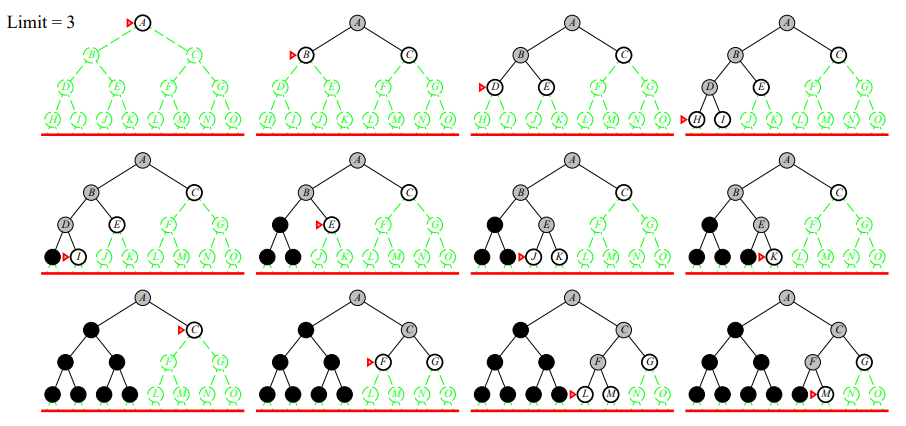
\includegraphics[width =123mm]{65_IDS_l2.png}\end{figure}
\end{frame}

%CAPITULO 3
%pagina 68
\begin{frame}{Propiedades de la Búsqueda de Profundización Iterativa}
    
    \\\textcolor{purple}{Completo??} SI
    \\\textcolor{purple}{Tiempo??} \textcolor{pink}{$(d+ 1)b^0+db^1+ (d-1)b^2 + ... + b^d= O(b^d)$}
    \\\textcolor{purple}{Espacio??}
        
\end{frame}

%Capitulo 3, presentación 69
\definecolor{Pink}{RGB}{255,0,131}
\definecolor{Purple}{RGB}{110,0,200}
\begin{frame}{Propiedades de la Búsqueda A Profundidad Iterativa}
    \small{ 
        \textcolor{Pink}{\underline{¿Completo?}}\, Si
        \\
        \textcolor{Pink}{\underline{¿Tiempo?}}\;\textcolor{Purple}{$(d+ 1)b^0+db^1+ (d-1)b^2 + ... + b^d= O(b^d)$}
        \\
        \textcolor{Pink}{\underline{¿Espacio?}}\;\textcolor{Purple}{$O(bd)$}
        \\
        \textcolor{Pink}{\underline{¿Optimo?}}\,
        \\
    }
\end{frame}

%slide 70

\definecolor{Pink}{RGB}{255,0,131}
\definecolor{Purple}{RGB}{110,0,200}
\begin{frame}{Propiedades de la Búsqueda A Profundidad Iterativa}
    \small{ 
        \textcolor{Pink}{\underline{¿Completo?}}\, Si
        \\
        \textcolor{Pink}{\underline{¿Tiempo?}}\;\textcolor{Purple}{$(d+ 1)b^0+db^1+ (d-1)b^2 + ... + b^d= O(b^d)$}
        \\
        \textcolor{Pink}{\underline{¿Espacio?}}\;\textcolor{Purple}{$O(bd)$}
        \\
        \textcolor{Pink}{\underline{¿Optimo?}}\, Sí, si el paso cuesta 1 
        \\
        Puede ser modificado para explorar un árbol con costo uniforme
        \\
        La comparasión númerica para \textcolor{Purple}{$b = 10$} y \textcolor{Purple}{$a = 5$}, la solución a la ultima hoja derecha
        \\
        \textcolor{Purple}{$N(IDS) = 50 + 400 + 3000 + 20000 + 100000 = 123450$}
        \\
        \textcolor{Purple}{$N(BFS) = 10 + 100 + 1000 + 10000 + 100000 + 999990 = 1111100$}
    }
\end{frame}

%CAPITULO 3
%pagina 71
\begin{frame}{Summary of algorithms}
    \begin{table}[htbp]
        \resizebox{12cm}{!} {
            \begin{tabular}{|l|c|c|c|c|c|} \hline
                \multicolumn{1}{|p{1.5cm}|}{\centering %
                Criterio} & \multicolumn{1}{p{4cm}|}%
                {\centering Búsqueda \\
                en anchura} & \multicolumn{1}{p{4cm}|}%
                {\centering Búsqueda \\
                de costo uniforme} & \multicolumn{1}{p{4cm}|}%
                {\centering Búsqueda \\
                en profundidad} & \multicolumn{1}{p{4cm}|}%
                {\centering Búsqueda \\
                en profundidad Limitada}
                & \multicolumn{1}{p{4cm}|}%
                {\centering Búsqueda \\
                en profundidad iterativa}
                \tabularnewline \hline
                Completo? & Si*     & Si*                              & No    & Si, Si $ l \geq d $ & Si    \\
                Tiempo    & b^{d+1} & b^ {\lceil {\frac{C}{E}} \rceil} & b^{m} & b^{l}               & b^{d} \\
                Espacio   & b^{d+1} & b^ {\lceil {\frac{C}{E}} \rceil} & bm    & bl                  & bd    \\
                Óptimo?  & Si*     & Si*                              & No    & No                  & Si*   \\  \hline
            \end{tabular}
        }
    \end{table}
\end{frame}

%Chap 3 pag 72
\begin{frame}{Estados repetidos}
    ¡La falla en la detección de estados repetidos puede convertir un problema lineal en
    uno exponencial!
    
    \begin{figure}
        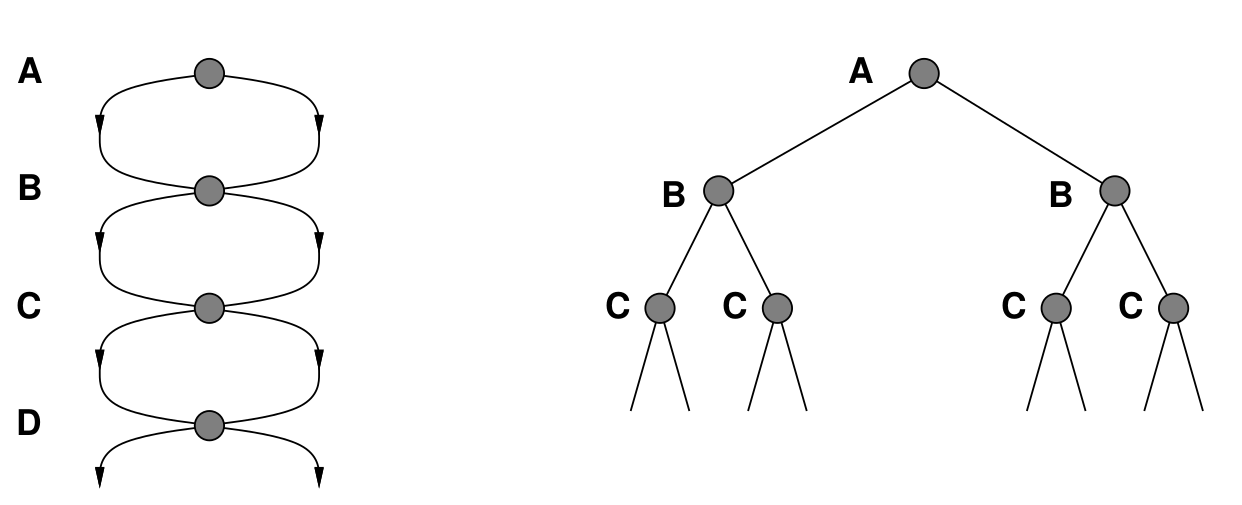
\includegraphics[scale=0.25]{72_chap3_pag72.png}
    \end{figure}
\end{frame}{}


\end{document} 